\chapter{Introduction} \label{chapter:Introduction}

This report focuses on the theoretical differences of how Natural Language Processing (NLP) models are implemented and subsequently how performance is affected with certain technical abilities, a key aspect of this report will demonstrate the question “does adding new to old bring enhancements?”. This chapter will cover the technical context of this project and report, the aims, objectives and introduce the domain in which this project lies. Natural language processing is subtopic topic covering and interconnecting computational theory, artificial intelligence/ machine learning and linguistics.

To consolidate the theoretical findings throughout technical chapters, this report will include two variants of a traditional NLP model that represents how a specific NLP technique is implemented. The aims of this project are to produce two machine learning models in which outline if and how traditional NLP techniques can be enhanced using modern theoretically driven techniques; the fundamental ideology of this project is to explore amalgamating NLP concepts and techniques to seek performance increases for dataset dependant models, the specific domain for this project is NLP in academia with the dataset being focused on Student Feedback Surveys. As seen in Chapter 2, we can expand our specific intention for this project and dataset to produce a novel NLP model on how to predict Student Feedback using the same techniques.

\section{Background and Context}

Natural Language Processing has been relatively overlooked during the boom of machine learning, its fundamentals have not changed as there has not been a reason to progress at the same rate as other areas in “Artificial Intelligence”, by adapting well---known theory, it is possible to progress the computational abilities of NLP. The background of this project is to bring modern approaches to older implementations with the justifications being student feedback surveys as the domain.

This project will be looking at areas from: Text and Speech Processing, Morphological Analysis, Syntactic Analysis and Lexical Semantics to give breakdowns of how they could function together to provide a potentially more efficient model.

\section{Project Aims and Objectives}

To successfully validate my project statement, there are several underlying implications that project aims must establish; the aims of this report are to compare the theory behind classical models and machine learning models of NLP and its subcategories of linguistics, such as grammar and text classification. This report will be corroborated using programming artifacts shown throughout, they will feature two NLP models, one of which demonstrates classical implementations on a given dataset and the other demonstrates an adapted form of a classical implementation with additional ML theory and techniques.

These aims will be achieved by meeting the following objectives:

\begin{itemize}
    \item Contrasting and comparing types of NLP techniques in a specific domain.
    \item Research and provide results for adding ML techniques to a traditional method.
	\item Compare older methods to modern methods.
	\item Speed advantages or disadvantages when combining different methods and implementations.
	\item Using research from this paper, compare POS tagging and word2vec with ML implementations for text classification and sentiment analysis using the results.
\end{itemize}

By meeting these objectives, this project will have highlighted a novel approach expored in \autoref{chapter:ProjectDesign} to text classification and minimising computational costs whilst having no detrimental effects to accuracy.

\section{Deliverable}

Project Deliverable: compilable Python object.

\section{Project Constraints and Risks}

The biggest constraint for such a problem---related project is one of time, including time management; the approach of this project is to reflect on current theory to understand how to implement a novel solution to a specific application’s domain, as implementations of Text---Classification are heavily theory dependant where each topic has a broad overview, it seems time will be of essence. A secondary constraint to this project may be inherited from a programmatic approach, whereby language features, libraries, or framework versions may have conflict.

\section{Risk Assessment and Mitigation}

This project's risks can be categorised as three major areas:

\begin{itemize}
	\item \textbf{\textit{Developer illness:}} Impact on project is subjective to the degree of severity.
	\item \textbf{\textit{Delays in communication:}} Due to COVID-19 and on-going pandemic, specifically "working from home".
	\item \textbf{\textit{Inadequate training data/ sample size:}} As a machine-learning based project, ample data is needed for successful training.
\end{itemize}

As seen in \autoref{appendix:AppendixPID}, there is a table outlining the risks and negative impact factors associated with this project from its initialization; this table is included for risks in \autoref{chapter:Introduction} as they have already been signed off and approved.

\begin{figure}[H]
    \centering
    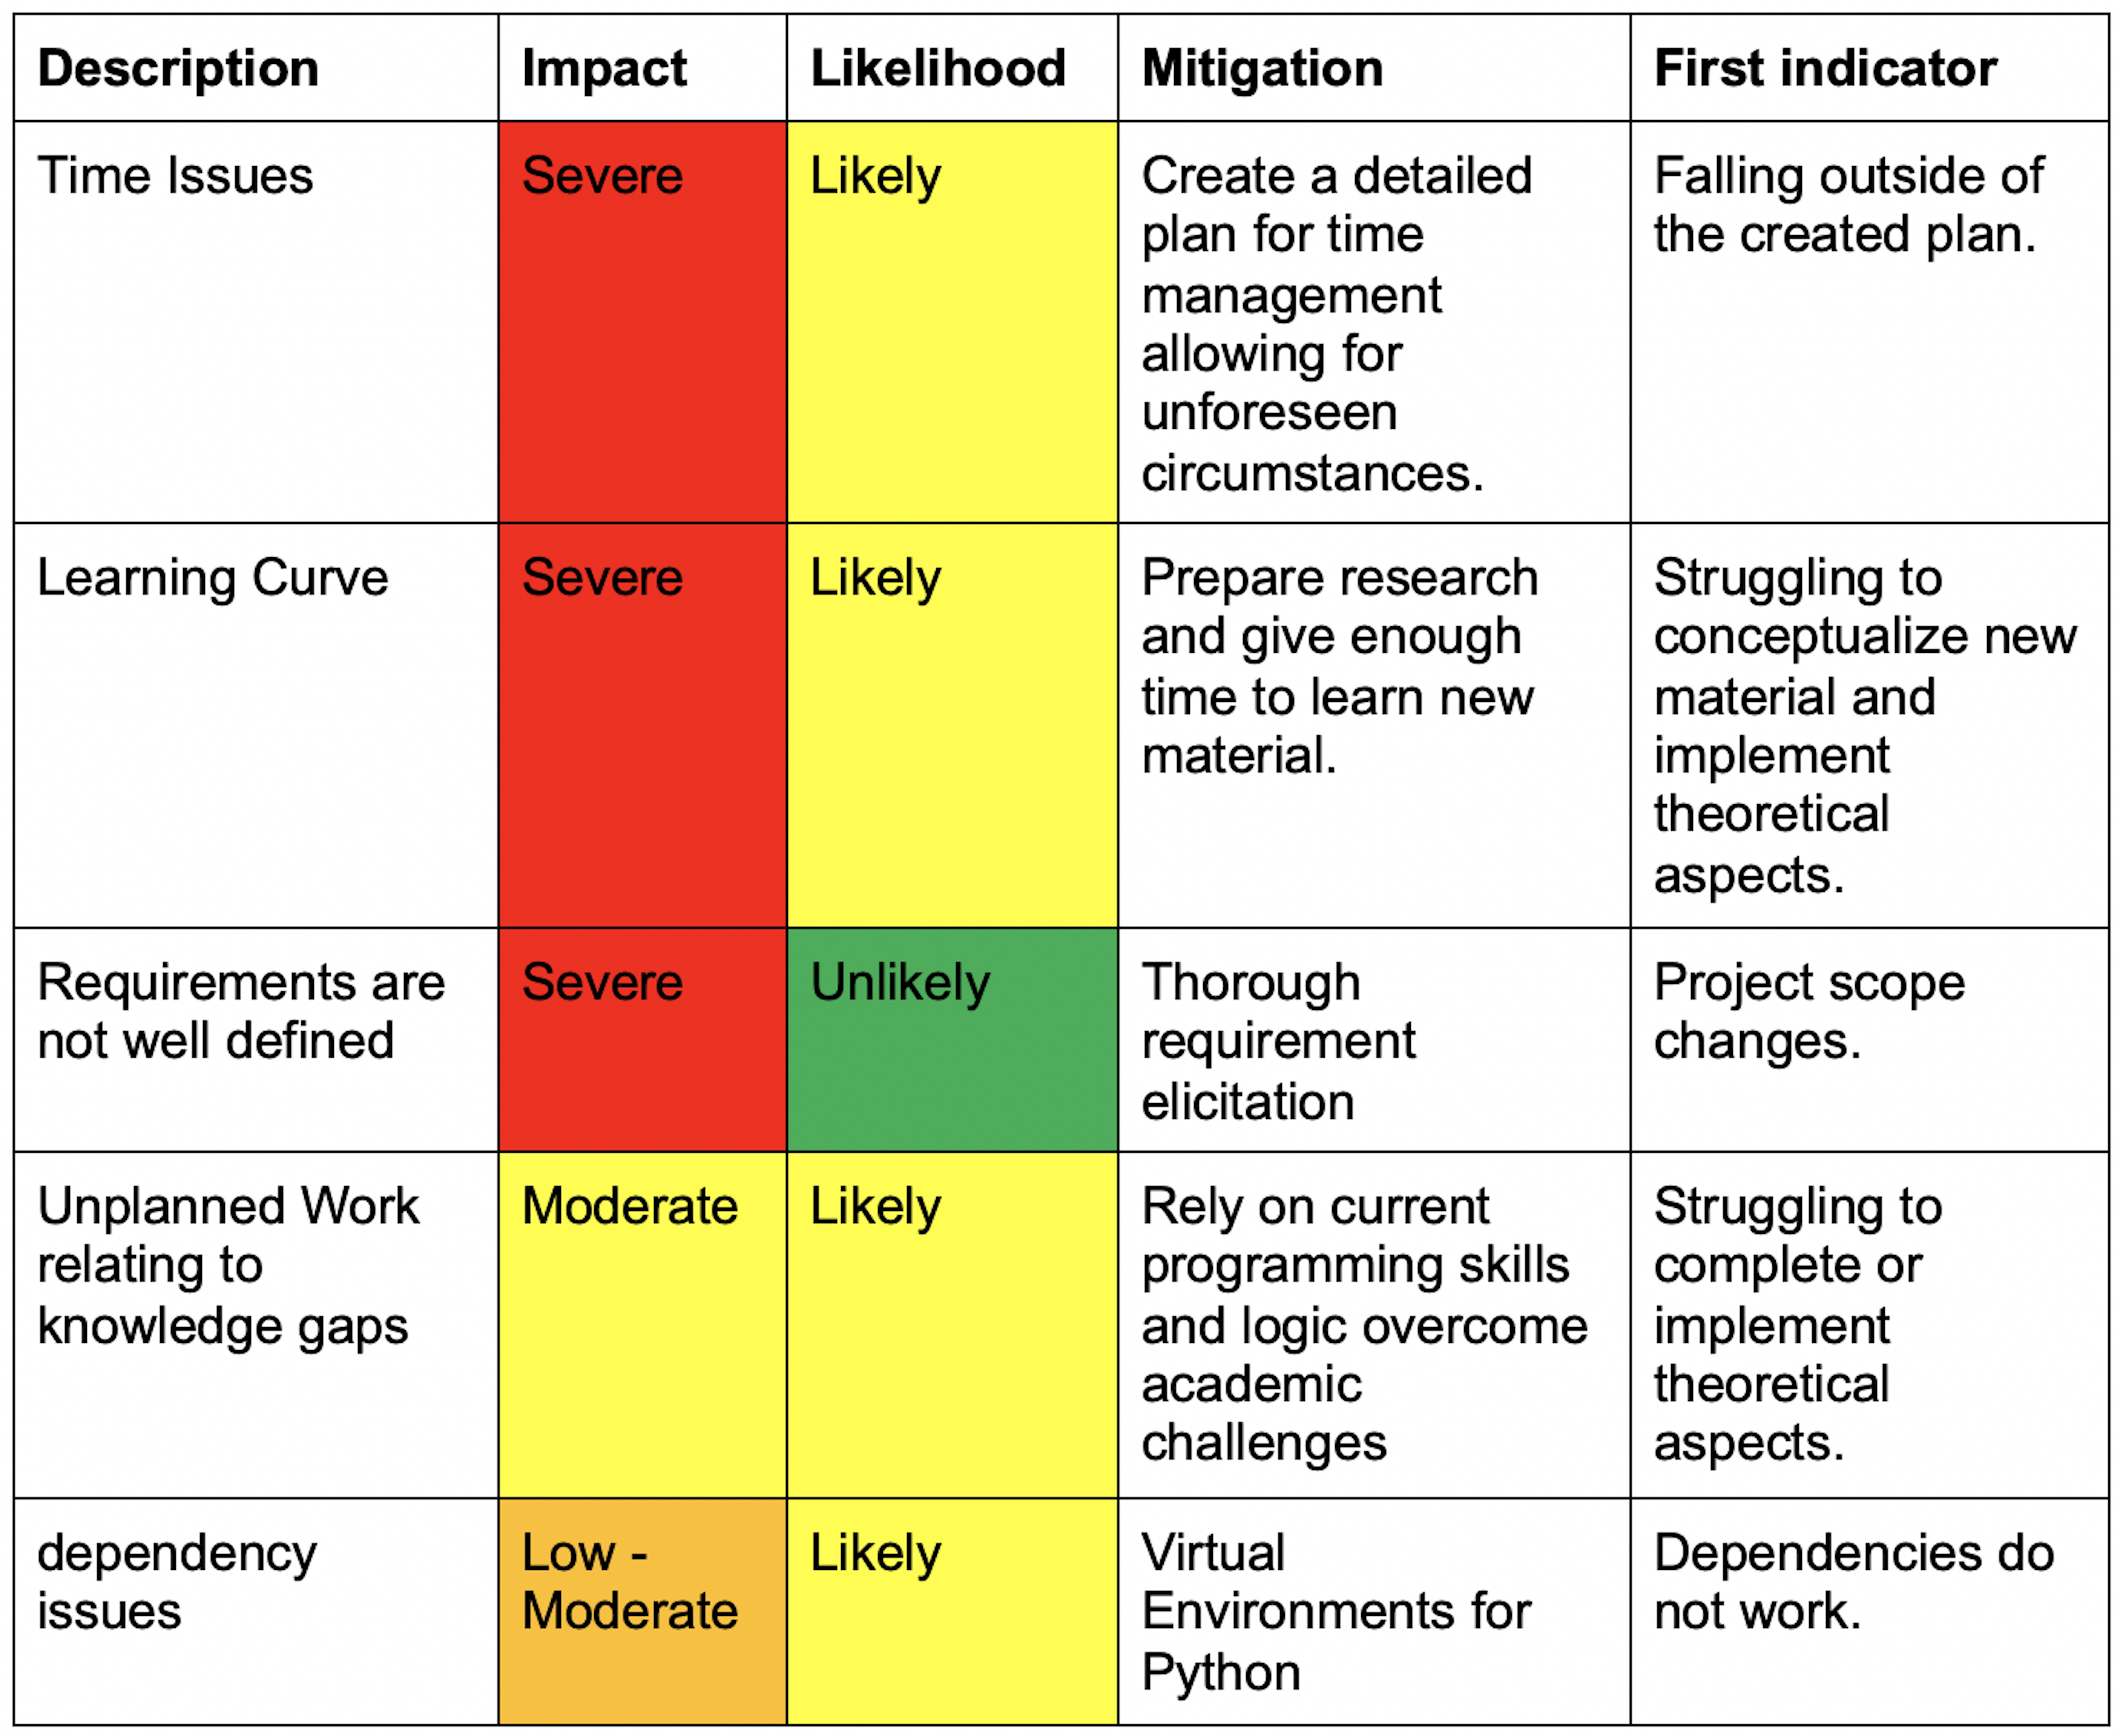
\includegraphics[width=\textwidth]{figures/chapter-1/PID-Risk-Table.png}
    \caption[PID-Risk-Table]{PID-Risk-Table.
    \label{fig:PID-Risk-Table}}
\end{figure}